\documentclass[12pt, twoside]{article}
\usepackage[letterpaper, margin=1in, headsep=0.2in]{geometry}
\setlength{\headheight}{0.6in}
%\usepackage[english]{babel}
\usepackage[utf8]{inputenc}
\usepackage{microtype}
\usepackage{amsmath}
\usepackage{amssymb}
%\usepackage{amsfonts}
\usepackage{siunitx} %units in math. eg 20\milli\meter
\usepackage{yhmath} % for arcs, overparenth command
\usepackage{tikz} %graphics
\usetikzlibrary{quotes, angles}
\usepackage{graphicx} %consider setting \graphicspath{{images/}}
\usepackage{parskip} %no paragraph indent
\usepackage{enumitem}
\usepackage{multicol}
\usepackage{venndiagram}

\usepackage{fancyhdr}
\pagestyle{fancy}
\fancyhf{}
\renewcommand{\headrulewidth}{0pt} % disable the underline of the header
\raggedbottom
\hfuzz=2mm %suppresses overfull box warnings

\usepackage{hyperref}

\fancyhead[LE]{\thepage}
\fancyhead[RO]{\thepage \\ Name: \hspace{4cm} \,\\}
\fancyhead[LO]{BECA / Dr. Huson / Geometry\\*  Unit 8: Congruence transformations\\* 3 January 2022}

\begin{document}

\subsubsection*{8.1 Homework: Translation \hfill CCSS.HSG.CO.A.5}
\begin{enumerate}
\item Do Now: A translation maps $A$ to $A'$, as shown, $A(3,1) \rightarrow A'(7,2)$.
\begin{multicols}{2}
  \begin{enumerate}
    \item What is the horizontal shift, how many squares right or left? \vspace{1.25cm}
    \item What is the vertical shift, how many squares up or down? \vspace{1.25cm}
    \item Apply the same translation to $C(1,4)\rightarrow C'(x,y)$. Label the point $C'$ as an ordered pair.
    \end{enumerate}
    \begin{flushright}
    \begin{tikzpicture}[scale=.635]
      \draw [help lines] (-1,-2) grid (8,6);
      \draw [thick, ->] (-1.2,0) -- (8.4,0) node [below right] {$x$};
      \draw [thick, ->] (0,-2.2)--(0,6.4) node [left] {$y$};
      \draw [fill] (3,1) circle [radius=0.05] node[below] {$A(3,1)$};
      \draw [fill] (7,2) circle [radius=0.05] node[below right] {$A'(7,2)$};
      \draw [->, dashed] (3,1)--(6.8,1.95);
      \draw [fill] (1,4) circle [radius=0.05] node[below] {$C(1,4)$};
    \end{tikzpicture}
    \end{flushright}
\end{multicols}

\item Vocabulary: A \emph{preimage} is \emph{mapped} to its \emph{image}. For example, triangle $ABC$ undergoes a transformation to make triangle $A'B'C'$.\\[0.5cm]
Translate $\triangle ABC$ by $(x,y) \rightarrow (x+6, y-2)$. Make a table of the coordinates and plot and label the image on the axes.
\begin{flushright}
    \begin{tikzpicture}[scale=.635]
    \draw [help lines] (-3,-2) grid (8,8);
    \draw [thick, <->] (-3.4,0) -- (8.4,0) node [right] {$x$};
    \draw [thick, <->] (0,-2.4)--(0,8.4) node [above] {$y$};  
    \draw [thick]
      (-2,3) node[below left] {$A$}--
      (-1,6) node[above left] {$B$}--
      (1,3) node[below] {$C$}--cycle;  
  \end{tikzpicture}
\end{flushright}

\newpage
\item Vocabulary: A translation is a \emph{rigid motion}, lengths and angles stay the same. \emph{Corresponding} parts are congruent. \\[0.5cm]
A translation maps triangle $KLM$ onto triangle $PQR$. \vspace{0.5cm}
  \begin{multicols}{2}
    \begin{tikzpicture}[scale=0.9]
      \coordinate [label=above left:$K$](A) at (95:2);
      \coordinate [label=below:$L$](B) at (0, 0);
      \coordinate [label=right:$M$](C) at (25:3.5);
      \draw [thick] (A)--(B)--(C)--cycle;
      \draw [thick, xshift=3cm, yshift=-2cm] (95:2) node[left]{$P$}--
      (0,0) node[below]{$Q$}--
      (25:3.5) node[right]{$R$}--cycle;
    \end{tikzpicture}\\
    Write each corresponding object.
    \begin{enumerate}
      \item $L \rightarrow$ \rule{2cm}{0.15mm}
      \item $\angle M \cong$ \rule{2cm}{0.15mm}
      \item $\overline {LM} \cong$ \rule{2cm}{0.15mm}
      \item Justify $\triangle KLM \cong \triangle PQR$. Use the words ``rigid motion" and ``translation''.
    \end{enumerate}
  \end{multicols}

\item A translation maps $A$ to $A'$, as shown, $A(2,1) \rightarrow A'(6,3)$.
\begin{multicols}{2}
  \begin{enumerate}
    \item What is the horizontal shift, how many squares right or left? \vspace{1.25cm}
    \item What is the vertical shift, how many squares up or down? \vspace{1.25cm}
    \item Apply the same translation to $C(1,3)\rightarrow C'(x,y)$. On the grid, mark and label the point $C'$ as an ordered pair.
    \end{enumerate}
    \begin{flushright}
    \begin{tikzpicture}[scale=.635]
      \draw [help lines] (-1,-2) grid (8,6);
      \draw [thick, ->] (-1.2,0) -- (8.4,0) node [below right] {$x$};
      \draw [thick, ->] (0,-2.2)--(0,6.4) node [left] {$y$};
      \draw [fill] (2,1) circle [radius=0.05] node[below] {$A(2,1)$};
      \draw [fill] (6,3) circle [radius=0.05] node[below right] {$A'(6,3)$};
      \draw [->, dashed] (2,1)--(5.8,2.95);
      \draw [fill] (1,3) circle [radius=0.05] node[below] {$C(1,3)$};
    \end{tikzpicture}
    \end{flushright}
\end{multicols}


\item A translation maps triangle $KLM$ onto triangle $PQR$. \\[0.5cm]
Fill in the blank with each corresponding object. \vspace{0.5cm}
  \begin{multicols}{2}
    \begin{tikzpicture}[scale=1]
      \coordinate [label=above left:$K$](A) at (95:2);
      \coordinate [label=below:$L$](B) at (0, 0);
      \coordinate [label=right:$M$](C) at (25:3.5);
      \draw [thick] (A)--(B)--(C)--cycle;
      \draw [thick, xshift=2cm, yshift=-3cm] (95:2) node[left]{$P$}--
      (0,0) node[below]{$Q$}--
      (25:3.5) node[right]{$R$}--cycle;
    \end{tikzpicture}

    \begin{enumerate}
      \item $K \rightarrow$ \rule{2cm}{0.15mm}
      \item $\angle L \cong$ \rule{2cm}{0.15mm}
      \item $\overline {KL} \cong$ \rule{2cm}{0.15mm}
      \item Which statement best justifies $\triangle KLM \cong \triangle PQR$? \\[0.5cm]
      A dilation centered at point $K$ with a scale factor $k=2$ was performed.\\[0.5cm]
      Since translation is a rigid motion, the triangle's size and shape remains the same.
    \end{enumerate}
  \end{multicols}


\item A translation maps $X(1,6) \rightarrow X'(3,9)$. What is the image of $Y(2,-2)$ under the same translation?


\item Translate $\triangle ABC$ by $(x,y) \rightarrow (x+5, y+2)$. Make a table of the coordinates and plot and label the image on the axes.
  \begin{flushright}
    \begin{tikzpicture}[scale=.635]
    \draw [help lines] (-3,-2) grid (8,8);
    \draw [thick, <->] (-3.4,0) -- (8.4,0) node [right] {$x$};
    \draw [thick, <->] (0,-2.4)--(0,8.4) node [above] {$y$};  
    \draw [thick]
      (-1,2) node[below left] {$A$}--
      (-1,4) node[above left] {$B$}--
      (2,5) node[above] {$C$}--cycle;  
    \end{tikzpicture}
  \end{flushright}


\item A translation maps $A$ to $A'$, as shown, $A(3,1) \rightarrow A'(6,3)$.
\begin{multicols}{2}
  \begin{enumerate}
    \item What is the horizontal shift, how many squares right or left? \vspace{1.25cm}
    \item What is the vertical shift, how many squares up or down? \vspace{1.25cm}
    \item Apply the same translation to $C(1,3)\rightarrow C'(x,y)$. On the grid, mark and label the point $C'$ as an ordered pair.
    \end{enumerate}
    \begin{flushright}
    \begin{tikzpicture}[scale=.635]
      \draw [help lines] (-1,-2) grid (8,6);
      \draw [thick, ->] (-1.2,0) -- (8.4,0) node [below right] {$x$};
      \draw [thick, ->] (0,-2.2)--(0,6.4) node [left] {$y$};
      \draw [fill] (3,1) circle [radius=0.05] node[below] {$A(3,1)$};
      \draw [fill] (6,3) circle [radius=0.05] node[below right] {$A'(6,3)$};
      \draw [->, dashed] (3,1)--(5.8,2.95);
      \draw [fill] (1,3) circle [radius=0.05] node[below] {$C(1,3)$};
    \end{tikzpicture}
    \end{flushright}
\end{multicols}

\item A translation maps triangle $ABC$ onto triangle $DEF$. \\[0.5cm]
Fill in the blank with each corresponding object. \vspace{0.5cm}
  \begin{multicols}{2}
    \begin{tikzpicture}[scale=1]
      \coordinate [label=above left:$A$](A) at (95:2);
      \coordinate [label=below:$B$](B) at (0, 0);
      \coordinate [label=right:$C$](C) at (25:3.5);
      \draw [thick] (A)--(B)--(C)--cycle;
      \draw [thick, xshift=2cm, yshift=-3cm] (95:2) node[left]{$D$}--
      (0,0) node[below]{$E$}--
      (25:3.5) node[right]{$F$}--cycle;
    \end{tikzpicture}

    \begin{enumerate}
      \item $A \rightarrow$ \rule{2cm}{0.15mm}
      \item $\angle B \cong$ \rule{2cm}{0.15mm}
      \item $\overline {AB} \cong$ \rule{2cm}{0.15mm}
      \item Which statement best justifies $\triangle ABC \cong \triangle DEF$? \\[0.5cm]
      Since translation is a rigid motion, the triangle's size and shape remains the same.\\[0.5cm]
      A dilation centered at point $A$ with a scale factor $k=2$ was performed.
    \end{enumerate}
  \end{multicols}

\item A translation maps $P(3,5) \rightarrow P'(2,9)$. What is the image of $Q(-3,2)$ under the same translation?

\item Translate $\triangle ABC$ by $(x,y) \rightarrow (x+4, y-1)$. Make a table of the coordinates and plot and label the image on the axes.
  \begin{flushright}
    \begin{tikzpicture}[scale=.75]
    \draw [help lines] (-1,-2) grid (8,8);
    \draw [thick, <->] (-1.4,0) -- (8.4,0) node [right] {$x$};
    \draw [thick, <->] (0,-2.4)--(0,8.4) node [above] {$y$};  
    \draw [thick]
      (1,2) node[below left] {$A$}--
      (1,4) node[above left] {$B$}--
      (4,2) node[below] {$C$}--cycle;  
    \end{tikzpicture}
  \end{flushright}

  
  





\end{enumerate}
\end{document}